\subsection{Chemical Kinetics, Equilibrium and Energetics}

\begin{enumerate}
	\item Hydrogen peroxide breaks down slowly to form water and oxygen; the reaction can be speed up by using a catalyst.
		\begin{enumerate}[topsep=0ex,itemsep=0ex,partopsep=1ex,parsep=1ex]
		\item[i)] How does the catalyst speed up the rate of reaction?
		\item[ii)] Name a possible catalyst that can be used to speed up the reaction.
		\item[iii)] Show that the catalyst always remains unchanged at the end of the reaction.
	\end{enumerate}
	
	\item Complete the following equations and determine the type of chemical reaction involved in each case.
		\begin{enumerate}[topsep=0ex,itemsep=0ex,partopsep=1ex,parsep=1ex]
		\item[i)] Zn$_{(S)}$ + H$_2$SO$_{4 (aq)} \rightarrow$
		\item[ii)] AgNO$_{3 (aq)}$ + NaCl$_{(aq)} \rightarrow$
		\item[iii)] N$_{2 (g)}$ + H$_{2 (g)} \rightarrow$
	\end{enumerate}
	
	\item In the graph below, curve 1 was obtained from the decomposition of 100 cm$^3$ of 1.0M hydrogen peroxide solution catalysed by manganese (IV) oxide, 2H$_2$O$_2 \rightarrow$ 2H$_2$O + O$_2$ \\
	\begin{center}
		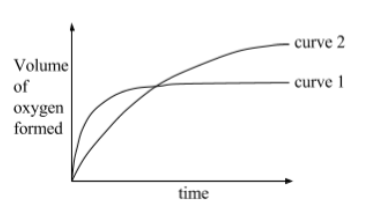
\includegraphics[width=0.5\textwidth]{./img/chem_III_kinetics_1.png}
	\end{center}
	Which alteration\slash change to the original experimental conditions would produce curve 2?
	\begin{enumerate}[topsep=0ex,itemsep=0ex,partopsep=1ex,parsep=1ex]
		\item[(A)] Lowering the temperature
		\item[(B)] Using less manganese (IV) oxide
		\item[(C)] Increasing the temperature
		\item[(D)] Adding some 0.1M H$_2$O$_2$ 
		\item[(E)] Using a different catalyst
	\end{enumerate}

	\item The reaction which produces methanol from carbon monoxide and hydrogen is represented by the equation CO$_{(g)}$ + 2H$_{2 (g)} \leftrightarrow$ CH$_3$OH$_{(g)}$ $\Delta$H = -94kJmol$^{-1}$. The reaction is carried out at high pressure to give a good yield of methanol
		\begin{enumerate}[topsep=0ex,itemsep=0ex,partopsep=1ex,parsep=1ex]
		\item[i)] Explain why increase in pressure gives a better yield of methanol
		\item[ii)] The value of $\Delta$H is negative. What does this tell about the reaction?
		\item[iii)] With a reason, state whether a high temperature or low temperature will give a better yield of methanol. 
	\end{enumerate}

\end{enumerate}









